\documentclass[12pt]{article}
\usepackage{eurosym}
\usepackage{times}
%\usepackage[T1]{fontenc}
\usepackage[bitstream-charter]{mathdesign}
\usepackage{natbib}
\usepackage{pdflscape}
\usepackage{afterpage}
\usepackage{textcomp}
\usepackage{amsmath}
\usepackage{dcolumn}
\usepackage{graphicx}
\usepackage{textcomp}
\usepackage{url}
\usepackage{xcolor}
\usepackage[colorlinks=true,citecolor=red!50!black,urlcolor=blue!50!black,linkcolor=red!50!black]{hyperref}
\setlength{\parindent}{10mm}
\usepackage[left=1in,top=1.25in,right=1.5in,bottom=1.25in]{geometry}
\usepackage{setspace}
\usepackage{sectsty}
\usepackage[title]{appendix}
%\renewcommand{\footnotesize}{\normalsize}
%\sectionfont{\normalsize}
%\subsectionfont{\normalsize}
%\setlength{\footnotesep}{0.6cm}

\title{The Modern Gatekeepers in Mass Media}

\author{Patrick Kraft\\PhD. Student\\Stony Brook University \and Yanna Krupnikov\\Assistant Professor\\Stony Brook University \and Kerri Milita\\Assistant Professor\\Illinois State University \and John Barry Ryan\\Assistant Professor\\Stony Brook University}

\begin{document}
\maketitle\thispagestyle{empty}

%150 word abstract
\begin{abstract}
The abstract goes here.
\end{abstract}

\bigskip
Prepared for presentation at the annual meeting of the Midwest Political Science Association, Chicago, April 8, 2016. The manuscript and code are available on GitHub: \url{https://github.com/pwkraft/nyt}.

\newpage
\clearpage
\setcounter{page}{1}
\begin{doublespace}
\section{Introduction}
I will write an introduction.

\section{The More Things Change...}

With technology, it is very tempting to herald the era following every advancement as fundamentally different from the era that proceeded it. The reality, however, is more nuanced than that. From the invention of the printing press to television to streaming services, each new technology has allowed creative people to tell their stories to a wider audience. Still, while each medium has its subtle differences in how it tells stories, there is something fundamental about drama and comedy that remains unchanged. That is what allows modern people to enjoy stories dating all the way back to ancient Greece and even before.

There is a similar tendency among some to say that social media has transformed how we consume political information. While their clearly some differences, we would argue it is foolish to assume the old theories no longer apply. Social media allows communication with larger numbers of people in dispersed locations--including people who have never been in the same room. At the same time, despite these differences, communication via social media is still, at its heart, one person sending messages to another person. In this fundamental way, it is no different from talking at a very large table.

To examine how much has changed in the era of Facebook and Twitter, we can examine how the "two-step flow" of information is different now. In the most basic form, the two-step flow would suggest that most people receive information from their friends, family, and co-workers who pay attention to the news media \citep{Katz1957}. If this were different, then we would expect that more people got their news from the primary sources--e.g., newspapers, television news, or internet news sites. If anything has changed, fewer people are receiving information directly from these news outlets necessitating the two-step flow of information even more \citep{Prior2005}.

With off-line social networks, there is a tendency towards political homophily \citep{XXXX}.  While it is unlikely that many people choose their discussion partners solely on the basis of politics, people do associate with individuals who are similar in terms of race, religion, education, and other factors which often correlate with political affiliations \citep{McPhersonSmithLovinCook2001}. Despite the tendency toward homophily, the complex patterns of social relations allows people to hold opinions different from some of their acquaintances \citep{HuckfeldtJohnsonSprague2004}. In fact, the more one talks about politics, the more likely they are to encounter disagreement \citep{HuckfeldtMendez2008}. This means that 21st century on-line social networks, which tend towards homophily but allow for some cross-cutting exposure, are not that different from the pre-internet social networks.

On-line social networks are larger than off-line social networks, but it is unclear how this difference matters. To describe some of the "friends" on social media as "weak" ties would stretch the definition of the concept. Granovetter \citeyearpar{Granovetter1973} noted that weak ties can provide information unavailable among an individual's intimate associates. Only a bold individual would ask for a job based on a Facebook post from someone he or she met a few times five years ago. Further, the most influential ties are those with some intimacy \citep{Kenny1998}. That is, the most important ties are those with whom one has a feeling of closeness. This feeling is more important than frequency of discussion or the duration of the connection \citep{MarsdenCampbell1984}. Hence, researchers suggest individuals should not look at the entire on-line social network if one wants to understand the truly influential connections. Rather, the meaningful social network is made of the individuals with whom one has direct communication--e.g., they comment on each other's photos \citep{XXXX}.

Finally, the most politically engaged are the most likely to share political information on social media \citep{XXXX}. The most politically engaged are also the most likely to discuss politics \citep{Huckfeldt2001}. The motivations in both instances are quite similar. As Ahn, Huckfeldt, and Ryan write \citeyearpar{AhnHuckfeldtRyan2014}, "We cannot expect opinion leaders to provide information that is balance, objective, and value free" (255). Opinion leaders discuss politics and post information about it on social media because they care about politics and they want to influence people. This is the most important way that the social communication is unchanged even with the internet. The modern two-step flow, like the two-step flow of previous eras, operates because individuals want to influence how people think about politics.

\section{Endogenous Agenda Setting}

To the extent that social media changes communication, it is not about interactions among peers. The major change involves how the news media interacts with the politically engaged members of the public. Whether referring to the news media as agenda setters or gatekeepers, the major theories of information flow in the 20th Century assumed that the media were the first movers in deciding what issues were important \citep{IyengarKinder1987}. Obviously, this view was always a bit oversimplified--as the "two-step flow" implies, the politically engaged members of the public acted as a second gatekeeper in regards to what stories most people heard. Further, 20th century editors would choose stories in part based on what stories they thought would sell newspapers \citep{XXXX}. For this reason, Thorson and Wells \citeyearpar{ThorsonWells2015} argue that we should think of modern gatekeeping in terms of "curated flows": journalists select certain stories to post on a website, engaged members select a subset of those to read, and they share an even smaller subset.

Social media adds another wrinkle to this agenda setting story. While 20th Century journalists had to anticipate which stories attract public attention and then receive noisy signals about the stories did capture the public, 21st Century journalists are able to quantify just how much attention a story is receiving. They then act on this information as they decide which stories to write about and which stories to feature \citep{XXX}. In this way, modern agenda setting is endogenous. Media gatekeepers set the agenda for the engaged members of the public. Engaged members of the public act as gatekeepers for everybody else sharing certain stories and not other. The media then writes more stories about the topics the engaged members of the public are sharing.

When engaged members of the public having greater say over the agenda, this has the potential to fundamentally change the news that makes the agenda. The most basic difference comes from the beliefs of the different agenda setting actors. In journalism, there are norms that encourage journalists to be neutral and, with some notable exceptions, many view their main role as informing the public \citep{XXXX}. The modern engaged public is marked by extreme positions \citep{Abramowitz2010} and their main goal is to persuade \citep{AhnHuckfeldtRyan2014}. This would suggest that there will be biases in terms of what stories are passed along. Typically, we think about biases in social communication as selective sharing of information in order to make one's own party look better \citep{AhnRyan2015,PietrykaND}. The more important biases in this case, however, may result from simply which types of stories receive attention.  

Hence, while this new form of agenda setting has many potential implications, this paper's goal is to explore a simple question: are the types of stories the news media values different from the types of stories the political engaged members of the public think are important? Is this the first question that any investigation in endogenous agenda setting must address. If the news media and the engaged public believe the same stories are important, then the feedback journalists receive now provides no new information to them. On the other hand, if the engaged public differs from journalists in its beliefs about what is important, then stories that would have previously been buried may begin to receive front page attention now that the journalists are more likely to follow the public.


\section{Data} 
The data for this study was collected from the website of \textit{The New York Times} between February 18 and April 28, 2015. We created a macro using Visual Basic that performed an exhaustive scrape of key areas of the website.\footnote{Standard web scraping platforms and programs (e.g., Outwit, rvest) were unable to extract all of the requested information, as the three subsections intermittently experienced html changes, such as an alteration in the font size or heading classification for a particular article.  Changes such as this will cause traditional web scraping programs to skip over these articles. Thus, it was necessary to write a macro that was customized to these three subsections of \textit{The New York Times} website. Using html parsing, we documented the source code for each subsection and noted common changes to the html over a course of three days. For instance, if a text-only article is replaced on the following day by one with embedded video, the source code will change to reflect that. The macro was programmed to run every 12 hours and to export the scraped material to an excel file with three tabs (one for each subsection). Every time the macro ran, it created an additional excel file (e.g., NYT01, NYT02, etc.).} The macro consisted of three web scrapers that extracted article title, author, date, time, and URL for (1) the front page of \textit{The New York Times}, which mirrors the lead stories on the hard copy of the newspaper, (2) the digital front page, which contains more stories than the hard copy of the front page, and (3) a subset of the front page that lists the top ten most viewed, most emailed, most shared articles.

This data collection allows us to analyze every story that appeared on the hardcopy and digital front pages of the \textit{New York Times}. It also allows us to see which types of stories the journalists see as more important--those that make the front page or receive a prominent placement on the digital front page. It also allows us to separate the agenda of the engaged public into separate categories in a way that is not capable with off-line social network research. We can see the stories they believe are important--those that make the most viewed list--and separate those stories from the stories they believe are the most important for other people to know--the most share on Facebook, Twitter, or via email.




\section{Description of Dataset}

In order to analyze the content of the NYT articles using the structural topic model approach presented by \citet{roberts2014structural}, I transformed the scraped articles to a reduced dataset where each unique article is included as a \textit{single} observation. Articles that appeared several times in the original raw collection (e.g. most tweeted article for several days) or through different channels (e.g. most tweeted and most viewed) were combined in a single observation. Overall, the reduced dataset contains 5504 \textit{unique} articles for subsequent analyses. Note that the number of articles is slightly lower than in the previous version (5592). I had to scrape the articles again in order to be able to calculate the readability indices (the previous scraping directly pre-processed the articles to omit punctuation etc.) and 88 articles could not be retrieved again in the second scraping. The missing articles were reuters/aponline press releases that were not available on the NYT website anymore.

For each observation, I created a vector of dichotomous variables indicating whether the respective article was included in each of the categories (emailed, facebook, etc.) at least once. Here is a sample of observations from this reduced dataset (article body, keywords, etc. are omitted). These variables represent the matrix of covariates that will be used in order to model differences in topical prevalence in the collection of documents.



\section{Initial Selection Model with 5 Topics}

We decided to focus our analysis on a subset of articles that contain political content. In order to select these articles, I estimated a first structural topic model with 5 topics using the \texttt{stm} package in \texttt{R} \citep[using spectral initialization, see][]{roberts2014structural,roberts2014stm}. In order to make the estimation computationally more tractable, I removed terms from the dictionary that only appeared in 10 articles or less. The following output presents an overview of the extracted topics by displaying words that are highly associated with the respective topic (using highest probability, FREX, Lift, Score, c.f. \citealt{roberts2014stm} for more details).

\begin{figure}
\caption{Highest probability words for topics}\label{fig:words}
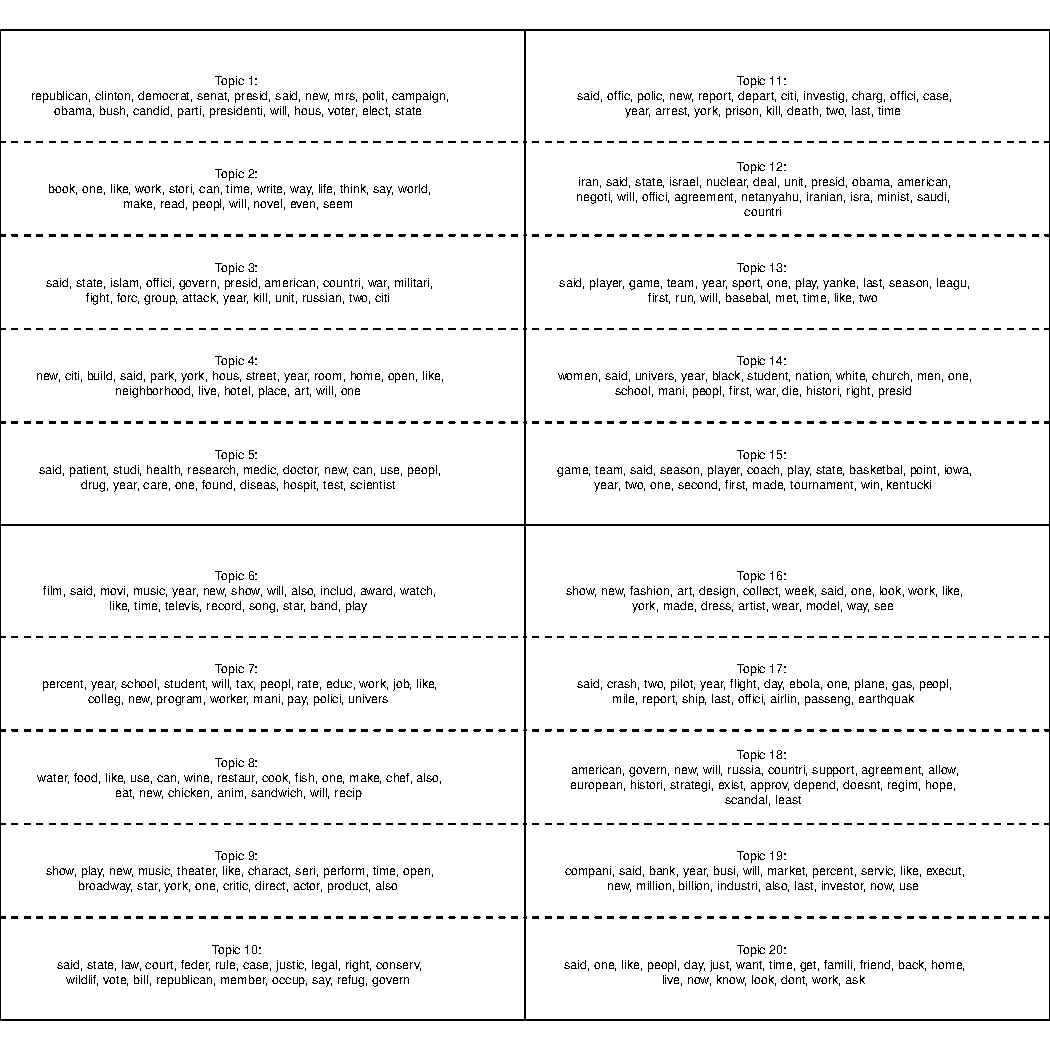
\includegraphics[width=\textwidth]{../calc/fig/words}
\end{figure}


The first topic clearly covers political issues and the US Presidential race. Topic 3 is mostly focused on conflicts, and topic 5 covers a mixture of economic, technology, and sports. Topics 2 and 4, on the other hand, cover cultural themes (movies, museum, fashion, etc.). The heterogeneity in topic 5 indicates that a total number of five topics is to small to properly characterize the corpus. Nevertheless, this broad categorization is sufficient to select a subset of articles related to political issues for the subsequent analyses. I omitted all articles that had the highest probability to belong to topic 2 and 4. Topic 5 was not omitted since it contains articles related to economic issues, which may well be politically relevant. As such, the filtering of political articles can be seen as conservative in the sense that we are more likely to include articles that are not clearly political rather than omitting articles that are. The reduced dataset consists of 3401 articles that were estimated to be most likely to belong to topics 1, 3, or 5.\footnote{It would also be possible to estimate a larger topic model using the entire set of articles and then only focus on topics that are clearly political. The substantive conclusions should not differ with either approach.}


\section{Results for Political/Economic Articles - 10 Topics}

After selecting the subset of articles that focus on political or economic issues, I estimated a second model with 10 topics. The following output again displays the topics along with highly associated words.


The following plot displays the proportions of each individual topic in the overall text body. I added descriptive labels for each topic.

\begin{figure}
\caption{Example for Topic Perspectives}\label{fig:prop}
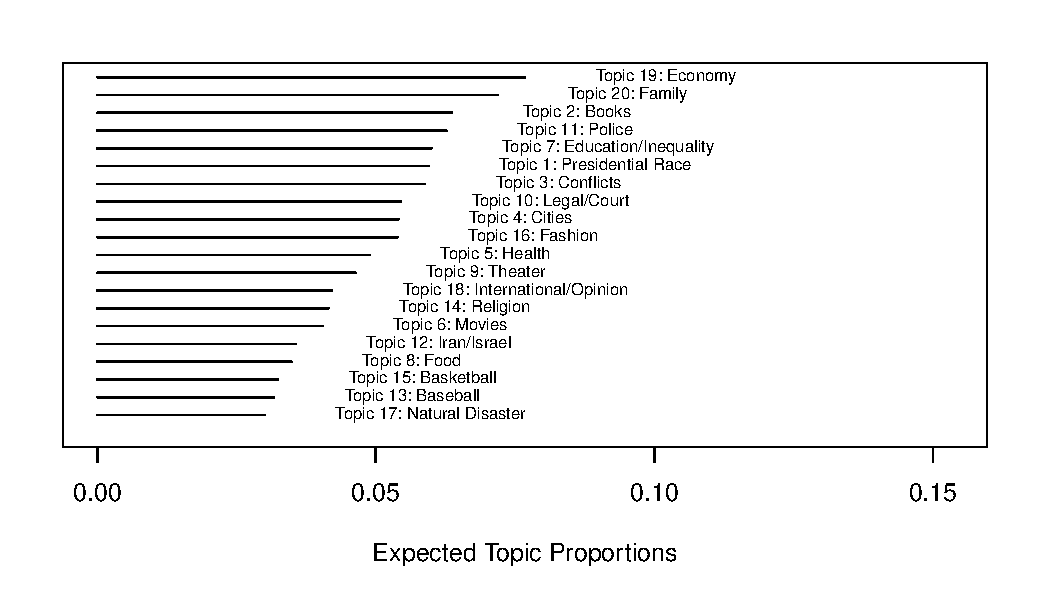
\includegraphics[width=\textwidth]{../calc/fig/prop} 
\end{figure}

Interestingly, the prevalence of topics in the corpus is quite evenly distributed. However, it should be kept in mind, that each observation in the document matrix can represent multiple instances of an article in the raw collection. The proportions presented here only describe the proportions in unique articles but does not take into account how often each of the articles was included originally (e.g. as most tweeted, or most viewed multiple times). 

We can also directly compare how certain words differentiate between topics. Consider for example topic 1 (presidential race) and topic 3 (international). The following plot displays how certain words are related to each of these topics. The size of the words is proportional to the frequency of occurence in the text, and the position on the x-axis describes whether the word is more related to either of the topics.

\begin{figure}
\caption{Example for Topic Perspectives}\label{fig:perspectives}
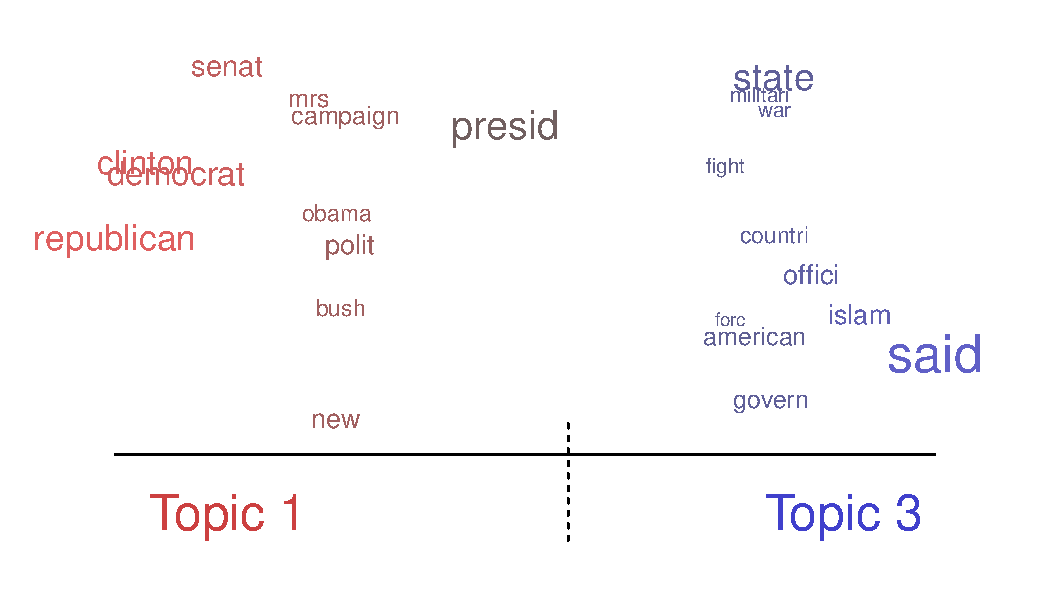
\includegraphics[width=\textwidth]{../calc/fig/perspective} 
\end{figure}

In this example, we can see that ``Clinton'' is clearly associated with topic 1 (presidential race), rather than topic 3 (international). The term ``president'' on the other hand, is mentioned frequently in both topics, but cannot be uniquey ascribed to either of the topics. This plausible finding provides some additional face validity for the topic model.


\section{Differences in Topic Proportions between Categories}

As described in \citet{roberts2014structural}, the structural topic model not only extracts topics from a collection of documents but also allows us to directly model the prevalence of topics in specific documents based on a matrix of meta-covariates. While it is also possible to use covariates in order to model differences in words used to describe certain topics, we only focus on differences with regard to \textit{how much} a topic is discussed in specific articles. The following figures display the change in the expected proportion to discuss individual topics for articles that were included in each of the categories or not.

As a first step, we examine topic distributions for content offered by the New York Times through different channels (printed front page vs. digital sections). Looking at the articles that appeared on the printed front page, we can see that the topics ``Technology'' and ``Health/Care'' are less likely to appear. The proportion of articles focusing on both topics is about 5 percentage points lower than in articles that do not appear on the printed front page. Other topics such as ``International'' or ``Police'' are sligthly more likely to be discussed in front page articles. This pattern is amplified when looking at the top news section of the digital edition. Again, ``Technology'' and ``Health/Care'' are less likely to appear (along with ``Sport''). On the other hand, articles in this category were more likely to discuss the presidential race, international affairs, police, as well as relations with Iran and Israel. The bottom section of the digital edition basically reverses the topic distribution in the top news section. Here, the proportion of articles related to technology, health, and sport is higher. Lastly, articles in the opinion section were more likely to discuss the Supreme Court and Iran/Israel.

\begin{figure}
\caption{Differences between categories}\label{fig:res_nyt_polecon}
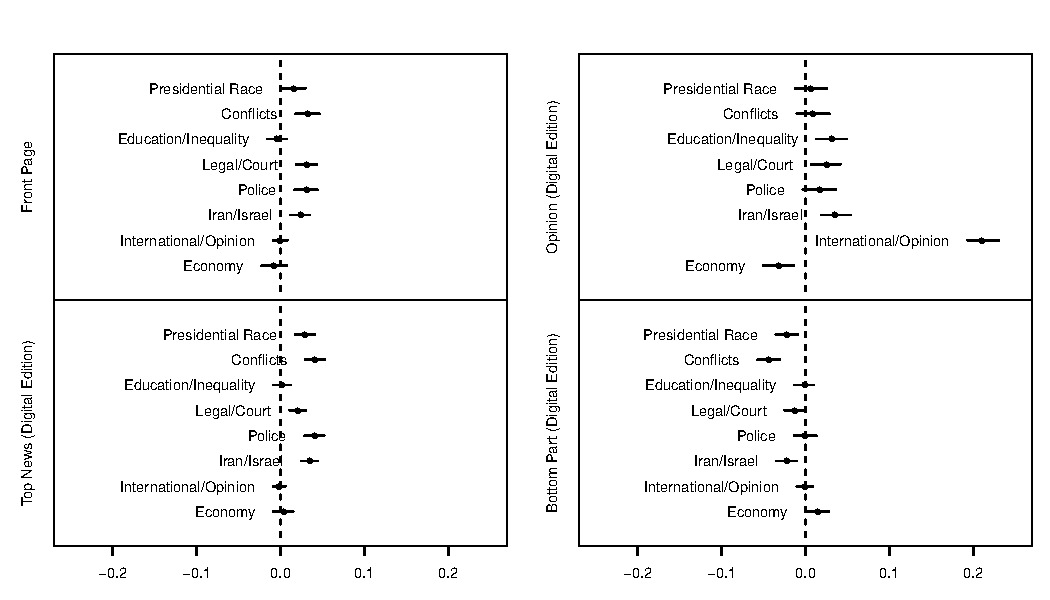
\includegraphics[width=\textwidth]{../calc/fig/res_nyt_polecon}
\end{figure}

Next, we compare topic distributions among articles that were most shared on different platforms. The figures reveal several interesting patterns. For example, we can see that articles that were most emailed were more likely to belong to the ``Health/Care'' topic but less likely to belong to political topics such as ``Presidential Race'', ``International'', or ``Supreme Court/Legal''. On the other hand, articles that were top shared on Facebook were more likely to belong to the topic ``Supreme Court/Legal''. Many articles in this topic discussed same-sex marriage and related Supreme Court decisions. As such, individuals who shared news content on Facebook were more likely to share articles related to marriage equality. Articles shared most on twitter, on the other hand, were more likely to discuss topics of ``Technology''. Overall, the results regarding shared content seem plausible in the context of underlying demographics of the population using each medium.

\begin{figure}
\caption{Differences between categories}\label{fig:res_share_polecon}
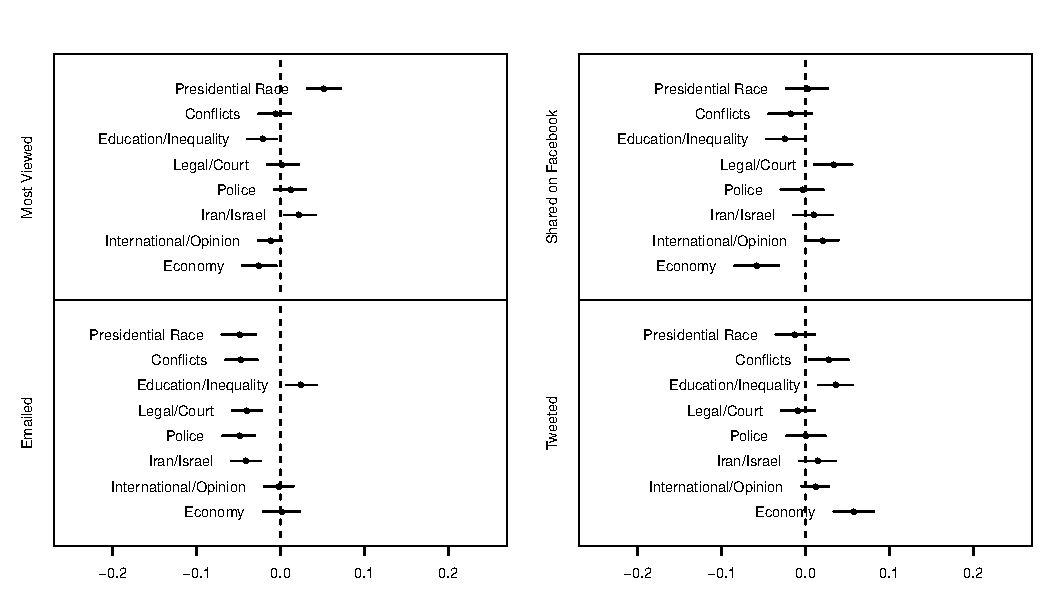
\includegraphics[width=\textwidth]{../calc/fig/res_share_polecon} 
\end{figure}

How do these patterns translate into views? The last plot (bottom right) of the previous figure displays change in topic proportions for articles that were most viewed. Articles in this category were more likely to discuss the presidential race, even though articles in this topic were not more likely to be shared on any platform. Other topics that were more likely in the most-viewed category are ``Police'' and ``Iran/Israel''. Interestingly, while articles about health were more likely to be emailed, they were less likely to be most viewed articles.


\section{Topic Proportions over Time}

We can also examine how the proportion of topics in each of the categories changes over time. Based on the topic model, I matched the estimated topic proportions for each article with the articles' dates of appearance. The following figure displays the aggregate topic proportions for a selection of political topics in each of the article categories from mid February till end of April. Especially the peaks in topic proportions are interesting here. For example, we see that the proportion of articles related to the topic ``Supreme Court/Legal'' in the top news category has a marked increase towards the end of the covered time period. Looking at the articles that were most viewed, we can identify several time points were the presidential race as well as the topic ``Police'' was more salient than other topics.


\begin{figure}
\caption{Topic proportions over time}\label{fig:series_nyt_main}
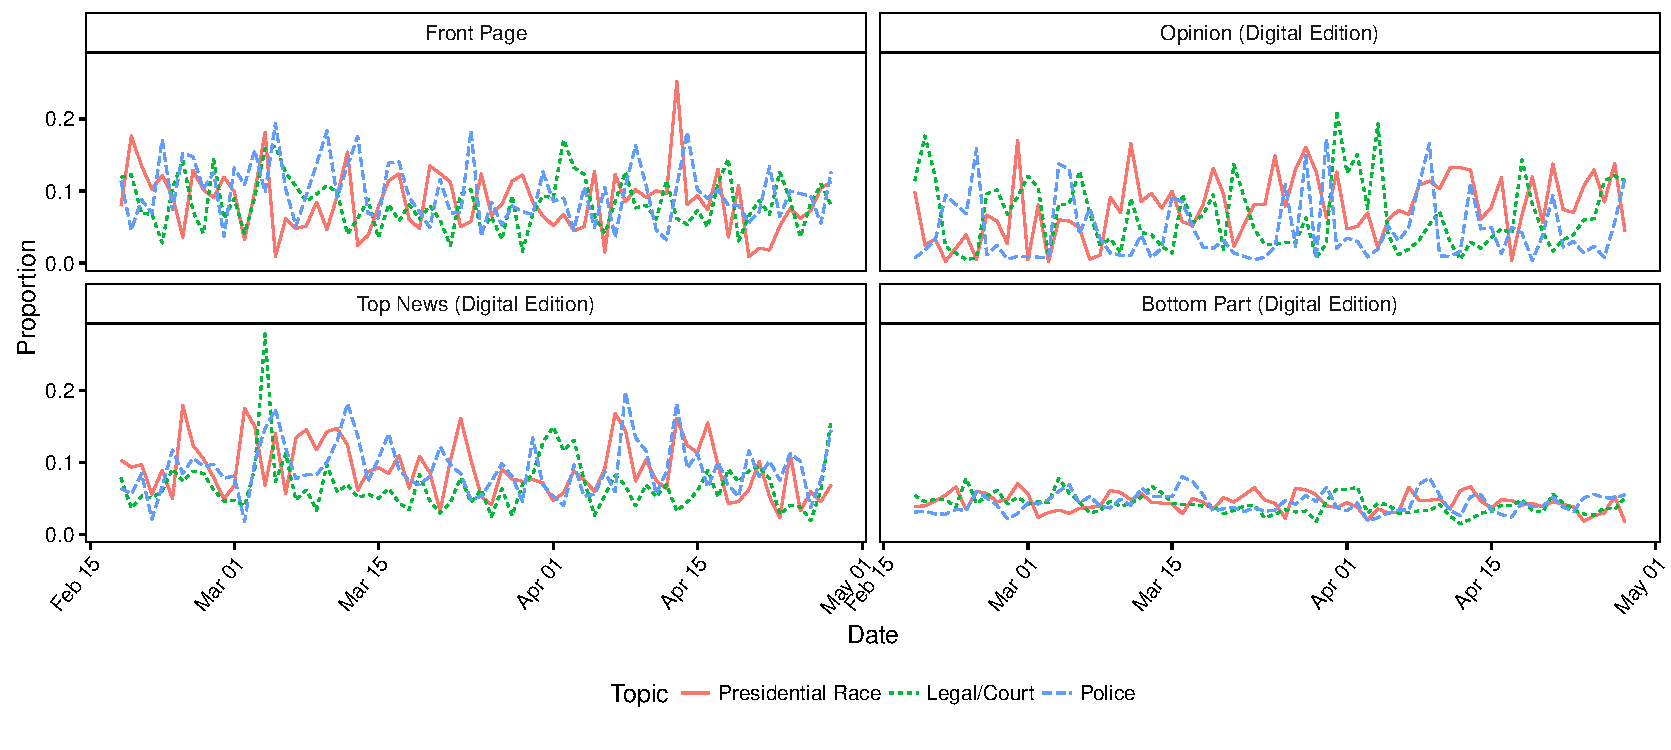
\includegraphics[width=\textwidth]{../calc/fig/series_nyt_main} 
\end{figure}

\begin{figure}
\caption{Topic proportions over time}\label{fig:series_share_main}
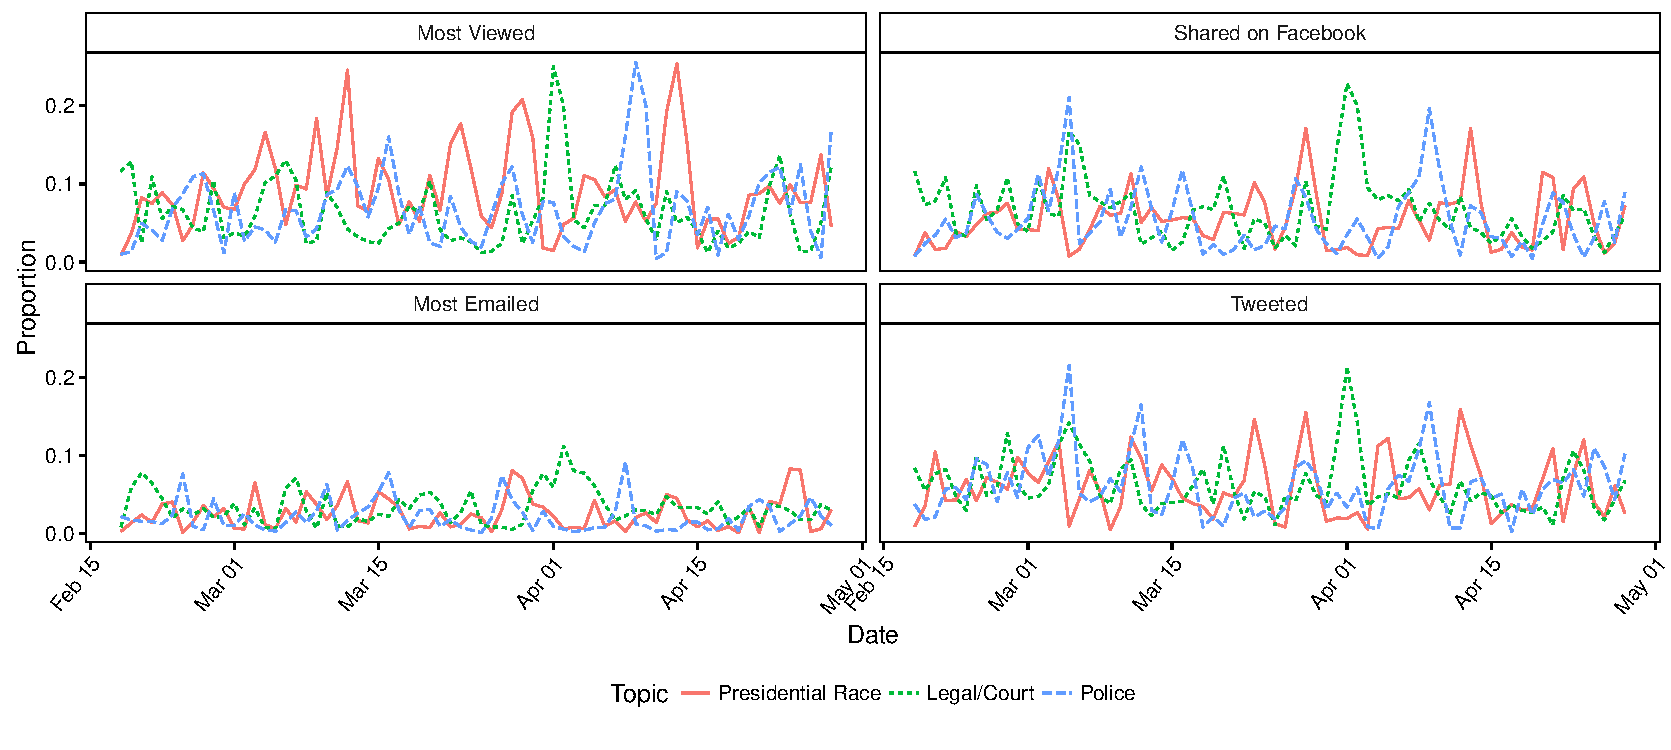
\includegraphics[width=\textwidth]{../calc/fig/series_share_main} 
\end{figure}

\section{Article Readability}

Another interesting question is whether there are structural differences between articles that determine whether they are more likely to be shared/most viewed etc. In order to examine whether the article complexity has any effect, I calculated the Automated Readability Index (ARI) for all articles (there are other readbility indices available, as well). The following figure displays the mean ARI scores for each article category. The ARI is supposed to map onto US grade years, so higher numbers indicate higher levels of difficulty. We can observe that articles that were most emailed are on average less complex/difficult to read than articles in any of the remaining categories.

\begin{figure}
\caption{Article Readability by Category}\label{fig:readability}
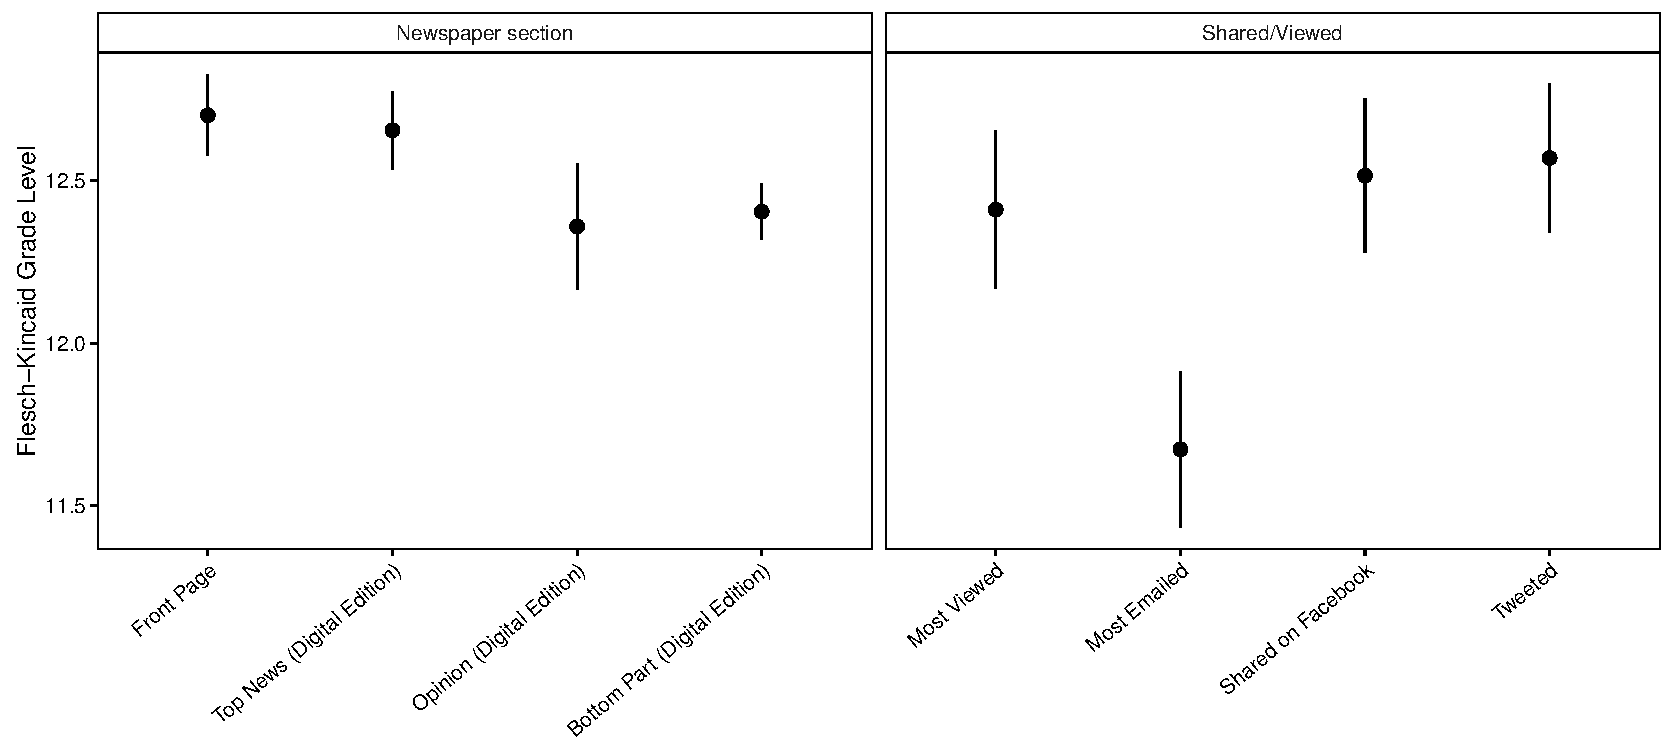
\includegraphics[width=\textwidth]{../calc/fig/readability} 
\end{figure}




\section{What stays in the loop}

As a last step, I started examining the order in which articles appear in each of the categories discussed so far. For example, it could be interesting to see whether articles are first shared and then become most viewed (or vice versa), or whether articles are potentially moved to the top news section after being shared a lot etc. I am not sure yet about the best way to model such patterns since the underlying data structure is relatively complex. To get a first impression, I selected all articles that were included in the dataset for mutiple days and calculated the proportion of article categories for each day since the first publication (most shared, top news etc.). The following figure displays the results.

\begin{figure}
\caption{What stays in the loop}\label{fig:switch}
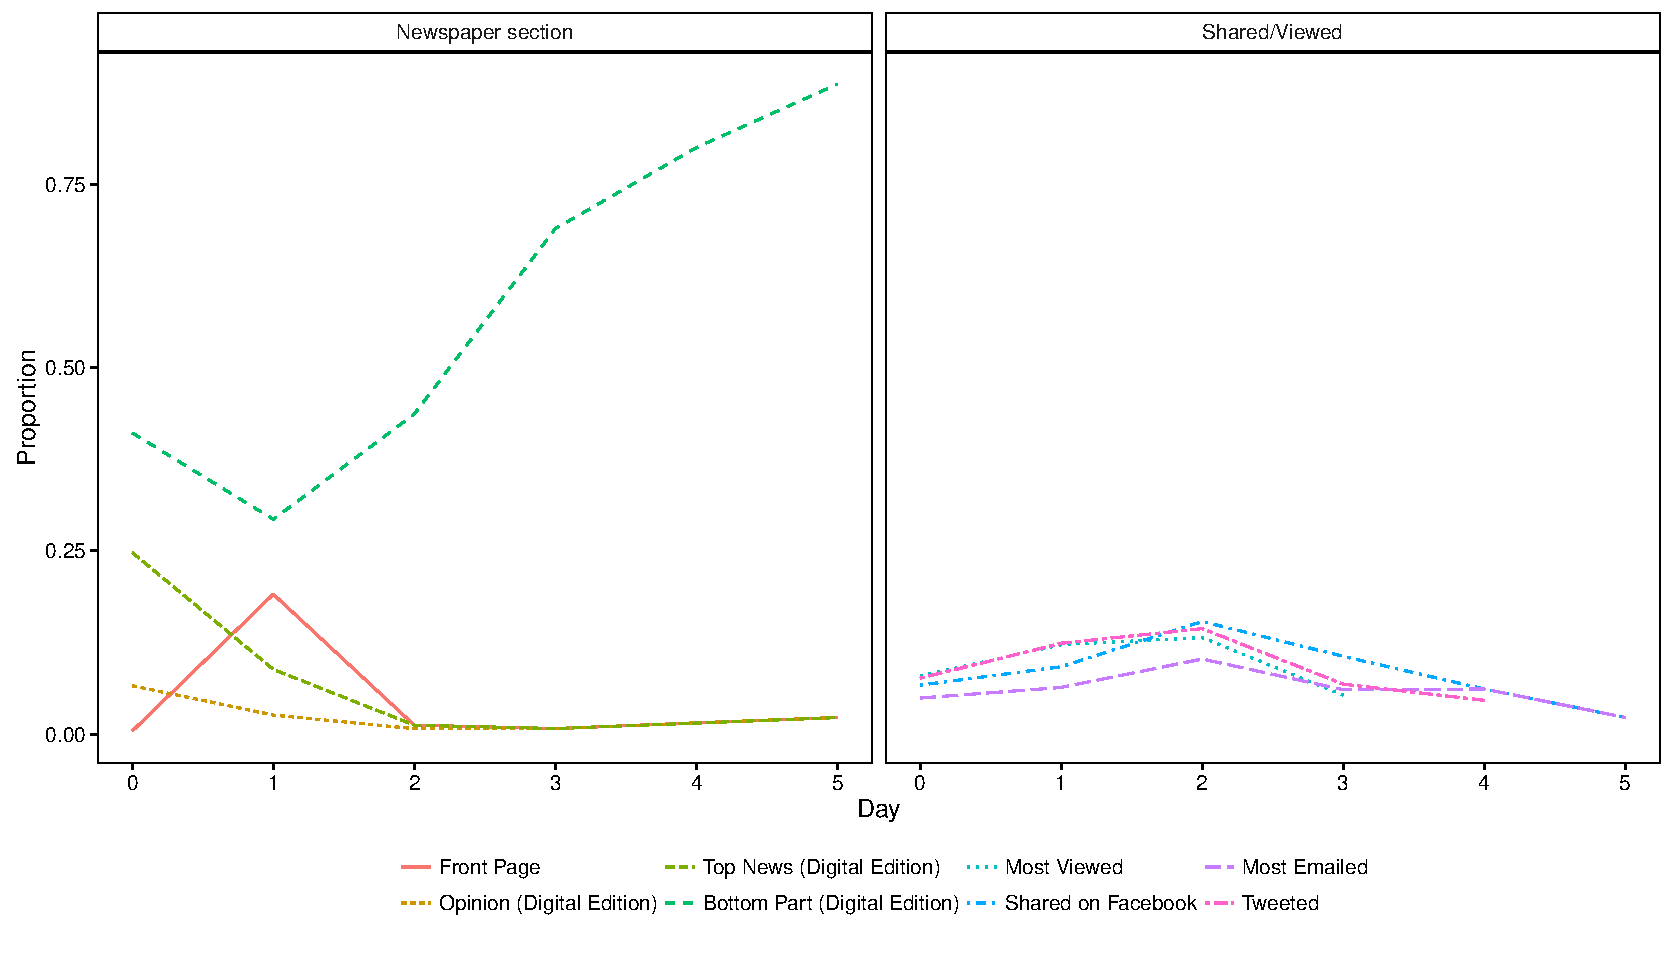
\includegraphics[width=\textwidth]{../calc/fig/switch} 
\end{figure}

On the first day of publication, most articles only appeared in the bottom section of the digital edition (about 40\%), or the top news section (about 25\%). Almost none of the articles that appear in the dataset for multiple times have been published on the printed front page first. Rather, they appear in print the day after being available online, as can be seen by the increase in the proportion of front page articles at day 1 (and the respective decrease in digital articles). The proportion of articles belonging to the most shared or most viewed categories increase throughout the first three days. While the differences are not very large, it appears that articles fall into the categories most tweeted and most viewed earlier than in the categories most emailed or most shared on facebook. Sharing on twitter and views might therefore preceed subsequent sharing on facebook and via email. However, it is worth noting again that these differences are relatively small and are so far only examined on an aggregate level. Nevertheless, these are interesting patterns that could be investigated further.


\clearpage
\section{Conclusion}


\vspace{1em}\noindent Possible subsequent steps:
\begin{itemize}\singlespacing
  \item investigate influence of other characteristics of articles (e.g. length of article)
  \item more analyses of temporal development on the level of individual articles
  \item set up hazard model, explain how long a topic stays in the cycle
\end{itemize}


\clearpage
\bibliographystyle{apsr2006}
\bibliography{JBRReferences.bib}


\end{doublespace}

\clearpage
\footnotesize\singlespacing
\appendices

\section{Topic Proportions between categories (all topics)}

\begin{figure}[h]
\caption{Differences between categories}\label{fig:res_nyt}
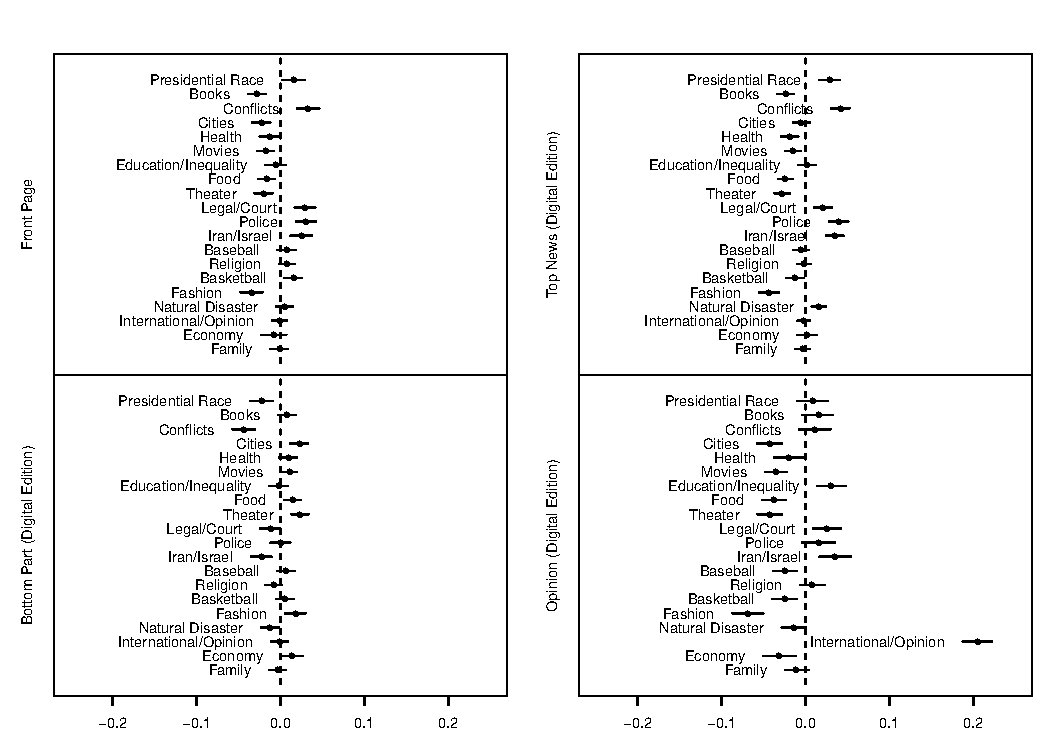
\includegraphics[width=\textwidth]{../calc/fig/res_nyt} 
\end{figure}

\begin{figure}[h]
\caption{Differences between categories}\label{fig:res_share}
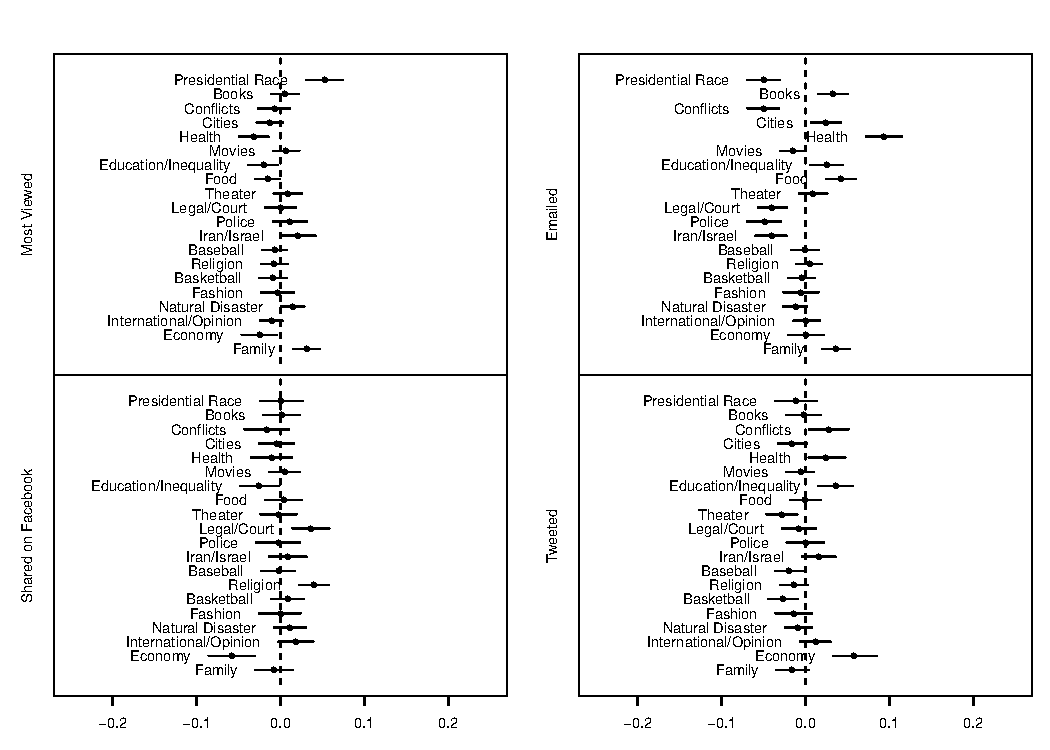
\includegraphics[width=\textwidth]{../calc/fig/res_share} 
\end{figure}


\clearpage
\section{Topic proportions over time (all topics)}

\begin{figure}[h]
\caption{Topic proportions over time}\label{fig:series_nyt}
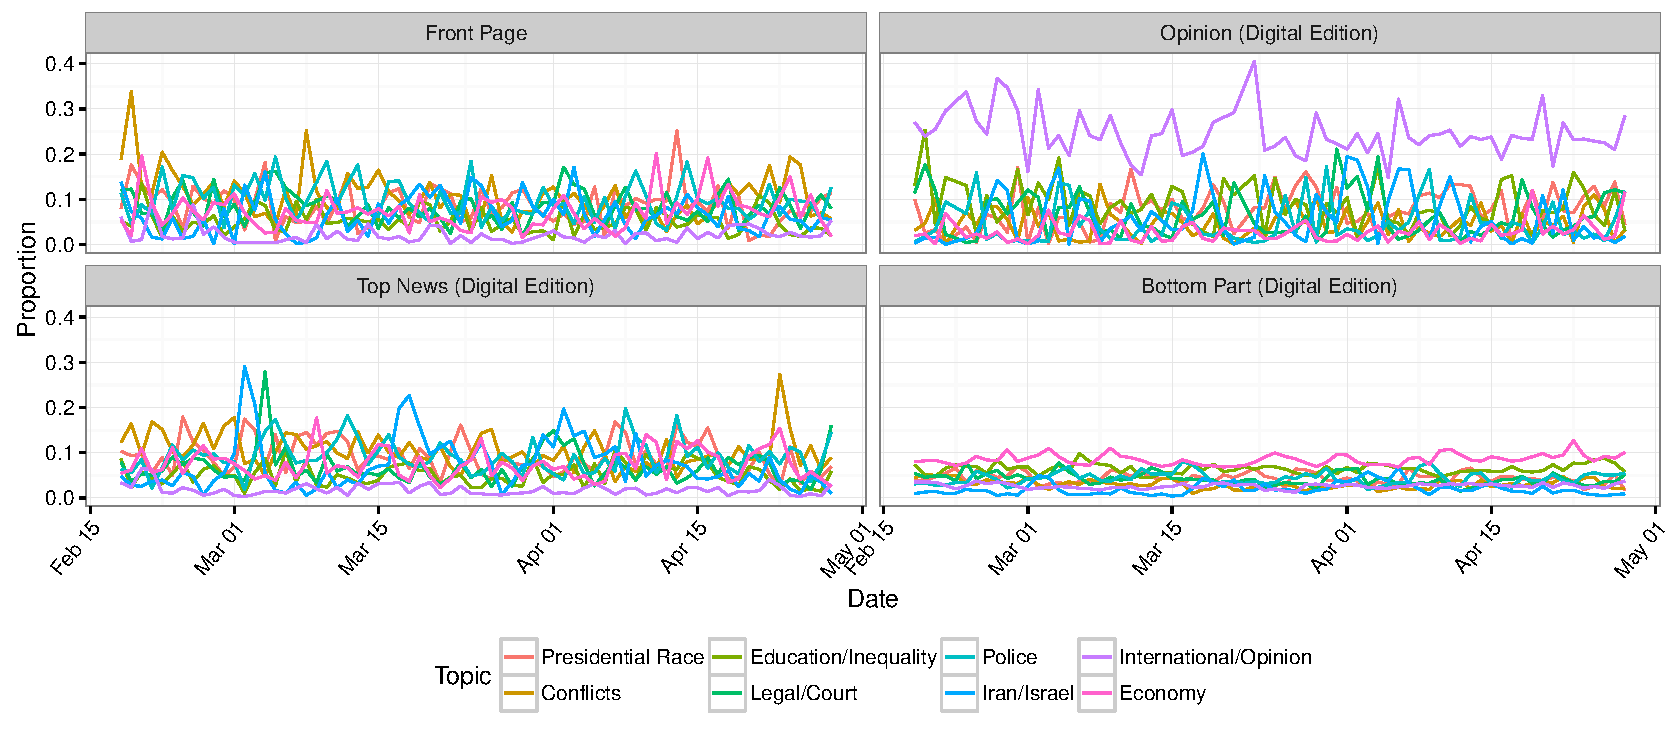
\includegraphics[width=\textwidth]{../calc/fig/series_nyt} 
\end{figure}

\begin{figure}[h]
\caption{Topic proportions over time}\label{fig:series_share}
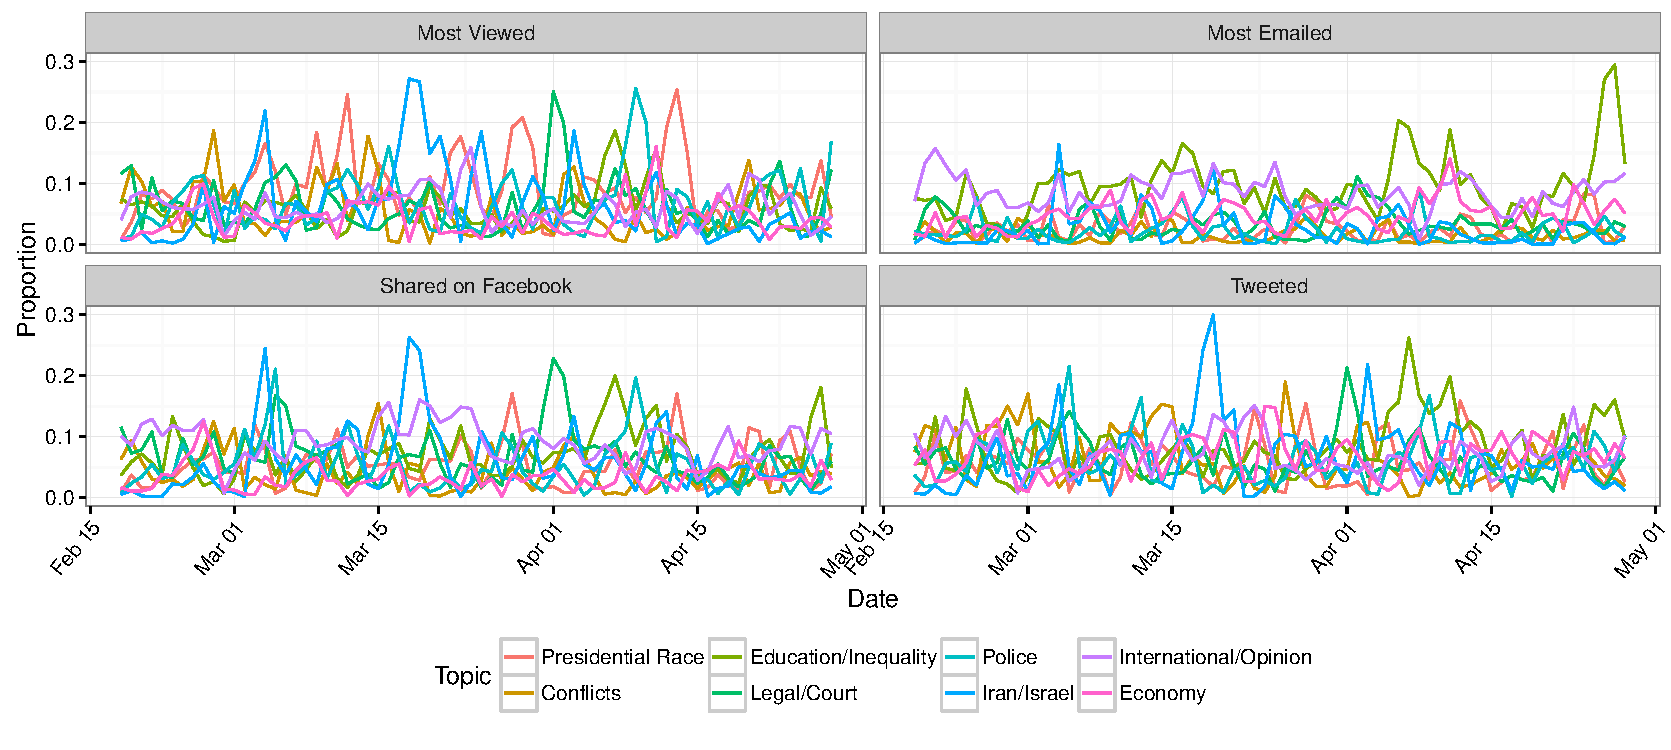
\includegraphics[width=\textwidth]{../calc/fig/series_share} 
\end{figure}



\end{document}